

\documentclass{llncs}
\usepackage[T1]{fontenc}
\usepackage[utf8]{inputenc}
\usepackage{currvita}
\usepackage{minted}
\usepackage{graphicx}
\usepackage{color}
\usemintedstyle{bw}
\setminted{fontsize=\small}





% *** CITATION PACKAGES ***
%
\usepackage{cite}
%\renewcommand\cite[1]{[[#1]]}

\usepackage{hyperref}
\hypersetup{
    % bookmarks=true,         % show bookmarks bar?
    unicode=true,          % non-Latin characters in Acrobat’s bookmarks
    pdftoolbar=true,        % show Acrobat’s toolbar?
    pdfmenubar=true,        % show Acrobat’s menu?
    pdffitwindow=false,     % window fit to page when opened
    pdfstartview={FitH},    % fits the width of the page to the window
    %pdftitle={},    % title
    %pdfauthor={Author},     % author
    %pdfsubject={Subject},   % subject of the document
    %pdfcreator={Creator},   % creator of the document
    %pdfproducer={Producer}, % producer of the document
    %pdfkeywords={keyword1, key2, key3}, % list of keywords
    %pdfnewwindow=true,      % links in new PDF window
    colorlinks=true,       % false: boxed links; true: colored links
    linkcolor=black,          % color of internal links (change box color with linkbordercolor)
    citecolor=black,        % color of links to bibliography
    filecolor=black,      % color of file links
    urlcolor=black,           % color of external links
    final=true
  }

\begin{document}
\title{Implementation of a Medical Quality Management System with Model Driven Architecture}

\titlerunning{Implementation of a QMS with MDA}

\author{Evgeny Cherkashin\inst{1,2,4,5}\and
  % Alexey Kopaygorodsky\inst{3,6}\and
Nikita Dorodnykh\inst{1}\and
Alexander Yurin\inst{1,5}\and\\
Ljubica Kazi\inst{4}\and
Alexey Shigarov\inst{1,2,4}\and
Vyacheslav Paramonov\inst{2,4}
%\and
%Boris Shevchenko\inst{6}\\[0.3em]
}

\tocauthor{Evgeny Cherkashin, Nikita Dorodnykh, Alexander Yurin, Ljubica Kazi, Alexey Shigarov, Vyacheslav Paramonov}

\authorrunning{Evgeny Cherkashin, Nikita Dorodnykh et al.}

\institute{Irkutsk Scientific Center of SB RAS, 134 Lermontov Street, 664033, Russia\and
Matrosov Institute for System Dynamics and Control Theory of SB RAS,\\ 134 Lermontov Street, 664033, Russia\and
%Melentiev Energy Systems Institute of SB RAS, 130 Lermontov Street, 664033, Russia\and
University of Novi Sad, Technical faculty "Mihajlo Pupin",\\ \DJ{}ure \DJ{}akovi\'ca bb,
 Zrenjanin, 23000, Serbia\and
Irkutsk State University, 20 Gagarina Avenue, 664002, Russia\and
National Research Irkutsk State Technical University,\\ 83 Lermontov Street, 664074, Russia\\
\email{eugeneai@icc.ru, tualatin32@mail.ru, ljubica.kazi@gmail.com}}

\maketitle

\begin{abstract} % 70-150 words
We consider problem of Quality Management System (QMS) development for Irkutsk Regional Oncological Dispancery.  The system is to organize the process of medical treatment of the patients according to the standard ISO 9001/2015.  QMS software carcass is synthesized as a result of a logical inference of a set of subgoals (a scenario) with a hierarchy of modules represented in the Logtalk programming language.  The source models are set of BPMN2.0, SysML and CMMN diagrams represented in XMI and other formats.  The models are imported and stored as ontologies A-boxes on an ontology server.  The models are transformed in special implementation-platform-oriented variants with following source code and initial data generation.  Additional data for the transformation are provided from Linked Open Data compliant sources.  Usage of such kind of Model Driven Architecture allows us to develop QMS on the abstract model level in most cased and involve domain specialist in the formal part of the development.


\keywords{quality management systems, model driven architecture, logical inference, linked open data}
\end{abstract}

\section{Introduction}
\label{sec:intro}

\begin{figure}[htb]
  \centering
  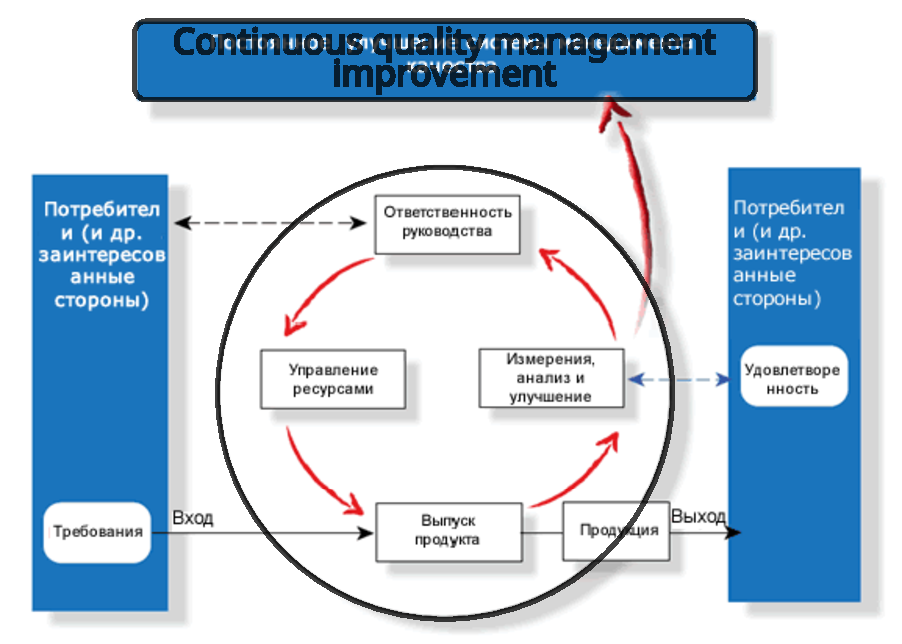
\includegraphics[width=0.8\linewidth]{qms-pics/iso9001.pdf}
  \caption{A general view on the ISO 9001/2015}
  \label{fig:iso9001}
\end{figure}

\section{Related research and technologies}
\label{sec:related}



\section{Acknowlegements}
\label{sec:acks}

The results are obtained with the partial support of the following projects:
\begin{itemize}
\item Irkutsk scientific center of SB RAS No 4.1.2;
\item The Council for grants of the President of Russian Federation, state support of leading scientific schools of the Russian Federation (NSH-8081.2016.9). %;
%\item Russian Foundation for Basic Research No 17-07-01341.
\end{itemize}
The results obtained with the use of the network infrastructure of Telecommunication center of collective use "Integrated information-computational network of Irkutsk scientific-educational complex" (\url{http://net.icc.ru}).

\begin{thebibliography}{99}
\bibitem{e}
\end{thebibliography}
\end{document}







%%% Local Variables:
%%% mode: latex
%%% TeX-master: "QMS-paper"
%%% End:
